\section{Gantt diagram}
\label{sec:gantt}

A Gantt diagram gives an overview of the overall time line of a project. The diagram orders items chronologically to easily show the projected state of the project at any given time. These items can represent milestones in the project, scrum sprints, deadlines and team downtime. 
The Gantt diagram for the project is shown in figure~\ref{fig:gantt}. The sprints are shown as blue rectangles and represent the teams working hours. The red rectangle indicates the trip to China that all the teams members went on in April. The blue diamonds indicate milestones, or deadlines for delivery of some major part of the project.


\begin{figure}[H]
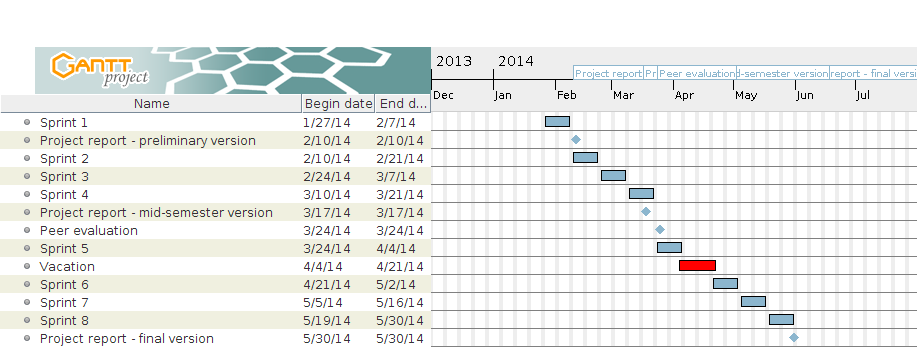
\includegraphics[width=\textwidth]{ch/prestudy/fig/gantt.png}
\caption{The Gantt diagram with sprints and milestones.}
\label{fig:gantt}
\end{figure}
